\documentclass[letter,11pt]{article}

\usepackage[spanish,es-nodecimaldot]{babel}
\usepackage[utf8]{inputenc}

\usepackage{lmodern}
\usepackage[T1]{fontenc}
\usepackage{textcomp}

\usepackage{framed}
\usepackage[svgnames]{xcolor}
\colorlet{shadecolor}{Gainsboro!50}

\usepackage[labelfont=bf]{caption}
\usepackage[shortlabels]{enumitem}
\usepackage{graphicx}
\usepackage{pstricks}

\usepackage{anysize}
\marginsize{3cm}{2cm}{2cm}{3cm}

\usepackage{url}
\usepackage{siunitx}
\usepackage{amsmath}
\usepackage{array}
\usepackage{alltt}

\usepackage{caption}
\newcommand{\source}[1]{\vspace{-11pt} \caption*{\small{\textbf{Nota:} {#1}}}}

\usepackage{fancyhdr}
\usepackage{lastpage}
\pagestyle{fancy}
\fancyhf{}
\fancyhead[LE,RO]{Laboratorio de Física Básica II}
\fancyfoot[CO,CE]{\thepage\ de \pageref{LastPage}}

\special{papersize=215.9mm,279.4mm}

\usepackage[
    pdfauthor={Carlos Eduardo Caballero Burgoa},%
    pdftitle={Laboratorio de Física Básica II},%
    pdfsubject={Medida de ruido ambiental},%
    colorlinks,%
    citecolor=black,%
    filecolor=black,%
    linkcolor=black,%
    urlcolor=black,
    breaklinks]{hyperref}
\usepackage{breakurl}

\newcommand{\blankpage}{
\newpage
\thispagestyle{empty}
\mbox{}
\newpage
}

\renewcommand{\arraystretch}{1.2}

\title{Informe 6: Medida de ruido ambiental}
\author{Carlos Eduardo Caballero Burgoa \\
    \small{\href{mailto:200201226@est.umss.edu}{200201226@est.umss.edu}}
}
\date{\today}

\newenvironment{conditions}
  {\par\vspace{\abovedisplayskip}\noindent\begin{tabular}{>{$}l<{$} @{${}={}$} l}}
  {\end{tabular}\par\vspace{\belowdisplayskip}}

\begin{document}

\maketitle
\begin{center}
    \textbf{Grupo}: J2\\
    \textbf{Docente}: Ing. Milka Mónica Torrico Troche\\
    \textbf{Carrera}: Ing. Electromecánica
\end{center}

\begin{abstract}
Este documento detalla la medición y el calculo del nivel sonoro representativo
en una avenida concurrida de la ciudad de Cochabamba, se tomó muestras de la
intensidad sonora con un sonómetro en intervalos de $5$ segundos durante $5$
minutos; posteriormente se calculó el valor representativo el cual es:
$70.57 [dB]$, y finalmente se analizó a partir de los niveles recomendados de
contaminación acústica, los cuidados y peligros a tomarse en cuenta.
\end{abstract}

\section{Introducción}

\begin{figure}
\centering
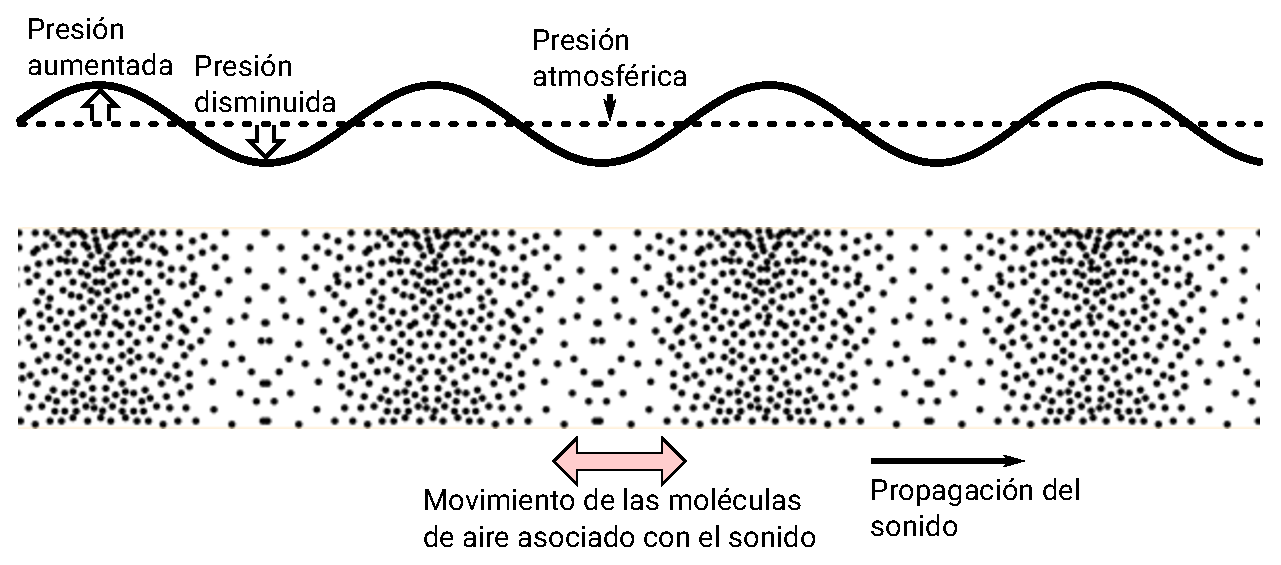
\includegraphics[width=0.60\textwidth]{resources/f1.eps}
\caption{Onda sonora.}
\label{figura1}
\source{El sonido y la audición (p. 3), \\
Constantino Pérez Vega. Universidad de Cantabria \cite{PEREZ}.}
\end{figure}

Una onda sonora es la propagación gradual de una perturbación caracterizada por
una vibración de las moléculas del medio alrededor de sus posiciones de
equilibrio (o estado de reposo) como puede observarse en la
\textbf{Figura \ref{figura1}}.
\\

A continuación de una perturbación, provocada en principio por una fuente
mecánica, las moléculas experimentan pequeños cambios de presión (presión
acústica). Las moléculas chocan entre ellas para transmitir la deformación
(perturbación) sufriendo de esta forma micro-desplazamientos. Estas moléculas
vuelven a su posición original cuando pasa la perturbación. El sonido es una
propagación de energía en un medio material sin transporte de materia
\cite{COCHLEA}.
\\

\begin{figure}
\centering
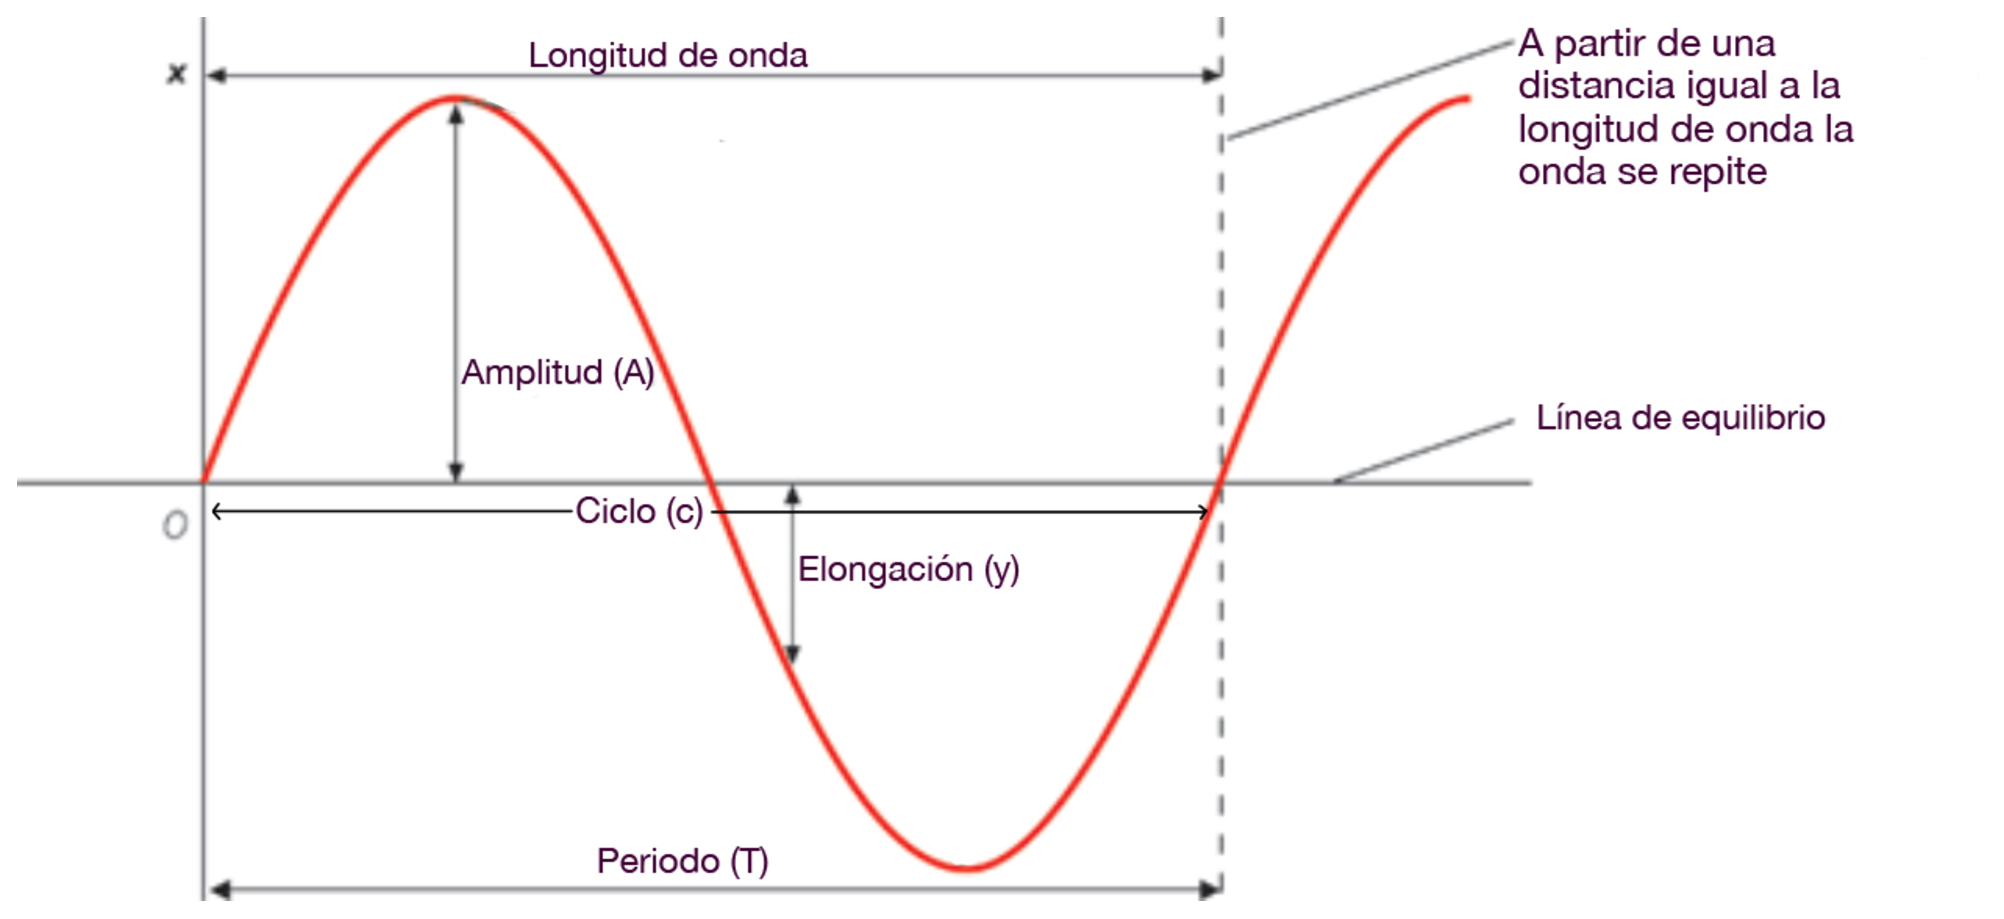
\includegraphics[width=0.75\textwidth]{resources/f2.eps}
\caption{Movimiento periódico con las magnitudes del sonido.}
\label{figura2}
\source{Nociones básicas sobre acústica musical \cite{MIGUELMORATEORGANOLOGIA}.}
\end{figure}

Las ondas sonoras más sencillas son las sinusoidales (o senoidales), las cuales
tienen frecuencia, amplitud y longitud de onda definidas
(\textbf{Figura \ref{figura2}}).
\\

El oído humano es sensible a las ondas en el intervalo de frecuencias de $20$ a
$20,000$ $[Hz]$, llamado \textbf{gama audible}, pero también usamos el término
``sonido'' para ondas similares con frecuencias mayores (ultrasónicas) y menores
(infrasónicas).
\\

Las ondas sonoras también pueden describirse en términos de variaciones de
presión en varios puntos (\textbf{Figura \ref{figura1}}). En una onda sonora
sinusoidal en el aire, la presión fluctúa por arriba y por debajo de la presión
atmosférica $P_a$ en forma sinusoidal con la misma frecuencia que los
movimientos de las partículas de aire. El oído humano funciona detectando estas
variaciones de presión. Una onda sonora que entra en el canal auditivo ejerce
una presión variable sobre un lado del tímpano; el aire del otro lado,
comunicado con el exterior por la trompa de \emph{Eustaquio}, está a presión
atmosférica. La diferencia de presión entre ambos lados del tímpano lo pone en
movimiento.
\\

La frecuencia de una onda sonora es el factor principal que determina el tono de
un sonido, la característica que permite clasificarlo como ``agudo'' o
``grave''. Cuanto más alta sea la frecuencia de un sonido (dentro de la gama
audible), más agudo será el tono percibido. La amplitud de presión también ayuda
a determinar el tono. Cuando un receptor compara dos ondas sonoras sinusoidales
con la misma frecuencia pero diferente amplitud de presión, la de mayor amplitud
suele percibirse más fuerte, pero también con un tono ligeramente más grave
\cite{Young&Freedman}.

\subsection{Nivel sonoro}

Dado que el sonido produce variaciones de la presión del aire debido a que hace
vibrar sus partículas, las unidades de medición del sonido podrían ser las
unidades de presión, que en el sistema internacional es el \emph{Pascal} ($Pa$).

\begin{equation*}
    1 [Pa] = 1 \left[\frac{N}{m^2}\right]
\end{equation*}
\vspace{0.10cm}

Sin embargo, el oído humano percibe variaciones de presión que oscilan entre 
$20 [\mu Pa]$ y $100 [Pa]$, es decir, con una relación entre ellas mayor de un
millón a 1, por lo que la aplicación de escalas lineales es inviable. En su
lugar se utilizan las escalas logarítmicas cuya unidad es el decibelio ($dB$) y
tiene la siguiente expresión \cite{SUPERINTENDENCIA}:

\begin{equation*}
    \beta = 20\cdot log_{10}\left(\frac{P}{P_0}\right) [dB]
\end{equation*}
\vspace{0.10cm}

Donde:

\begin{conditions}
\beta & Número de decibeles. \\
P     & Presión que se está midiendo. \\
P_o   & Presión de referencia. \\
\end{conditions}

Se utiliza esta escala logarítmica porque la sensibilidad que presenta el oído
humano a las variaciones de intensidad sonora sigue una escala aproximadamente
logarítmica, no lineal. Por ello el belio ($B$) y su submúltiplo el decibelio
($dB$), resultan adecuados para valorar la percepción de los sonidos por un
oyente. Se define como la comparación o relación entre dos sonidos porque en los
estudios sobre acústica fisiológica se vio que un oyente, al que se le hace
escuchar un solo sonido, no puede dar una indicación fiable de su intensidad,
mientras que, si se le hace escuchar dos sonidos diferentes, es capaz de
distinguir la diferencia de intensidad.
\\

Como el decibelio es una unidad relativa, para las aplicaciones acústicas se
asigna el valor de $0 [dB]$ al umbral de audición del ser humano, que por
convención se estima que equivale a un sonido con una presión de $20$
micropascales, algo así como un cambio de la presión atmosférica normal de
$1/5 000 000 000$. Aun así, el verdadero umbral de audición varía entre
distintas personas y para una misma persona, depende de la frecuencia del
sonido. Se considera el umbral del dolor para el humano a partir de los
$140 [dB]$. Esta suele ser, aproximadamente, la medida máxima considerada en
aplicaciones de acústica \cite{WIKI1}.

Pueden apreciarse algunos valores representativos del nivel de intensidad del
sonido en la \textbf{Figura \ref{figura3}}.

\begin{figure}
\centering
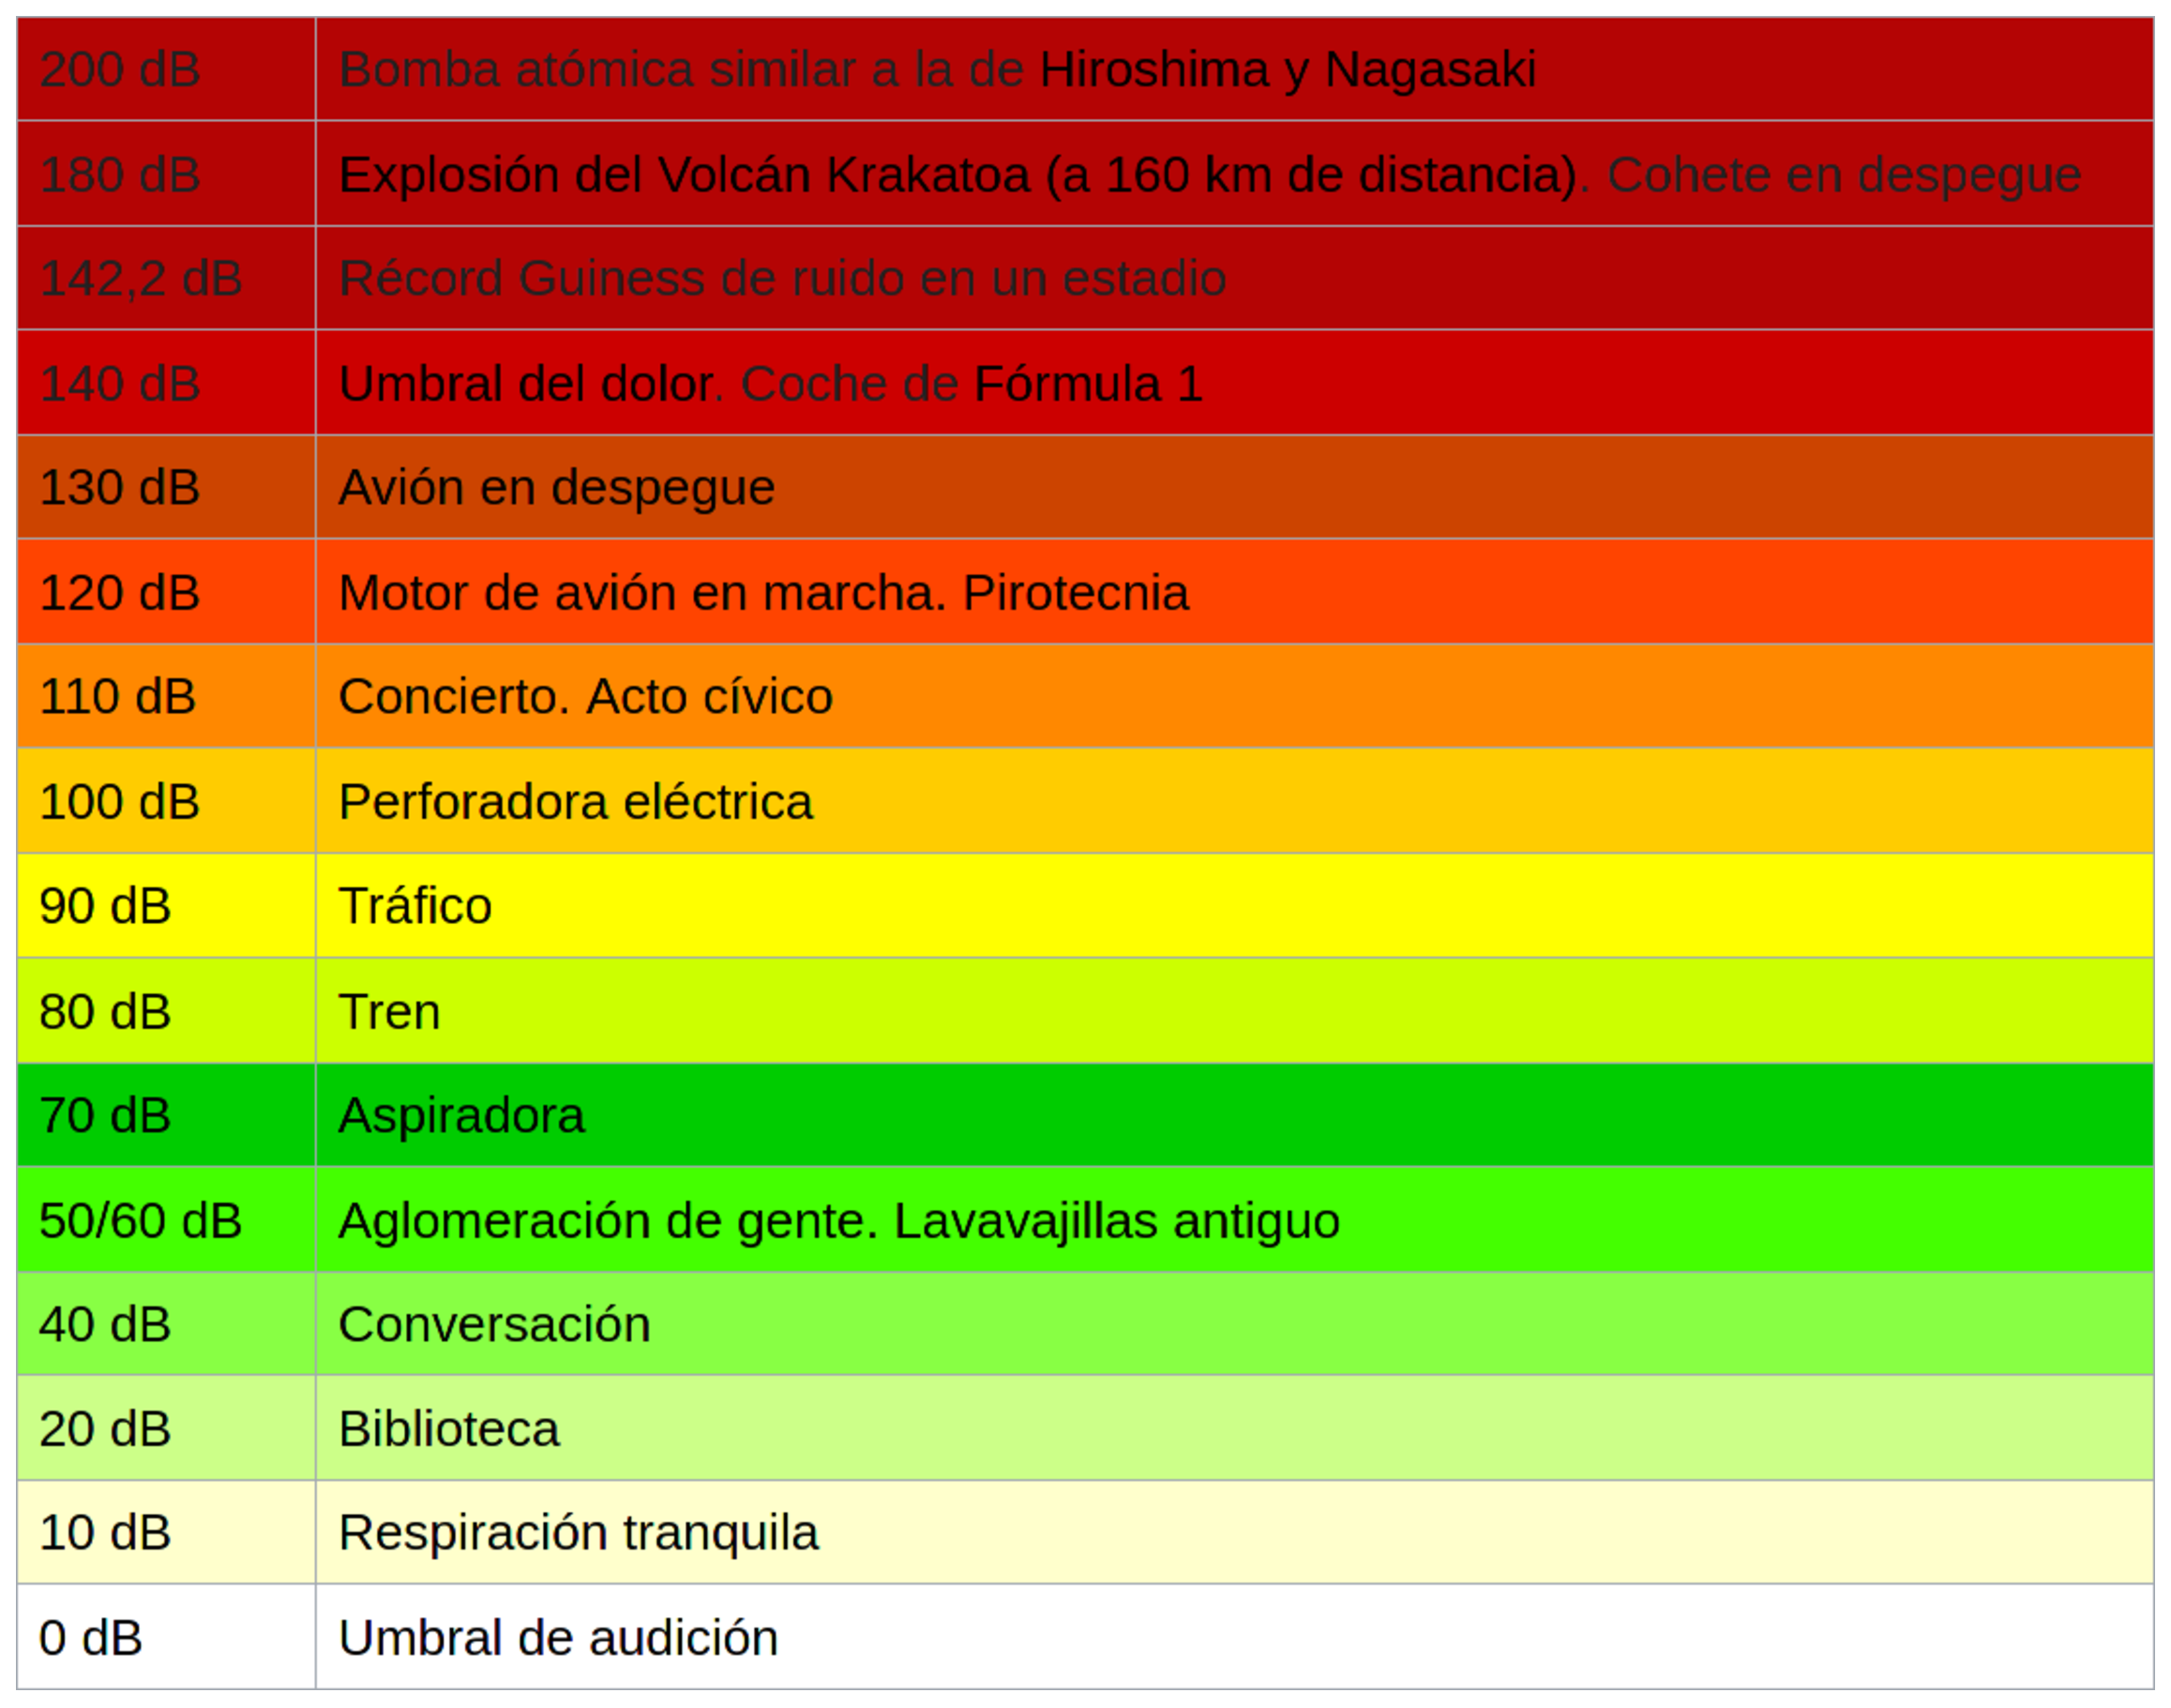
\includegraphics[width=0.72\textwidth]{resources/f3.eps}
\caption{Niveles de intensidad de sonido de diversas fuentes.}
\label{figura3}
\source{Adaptado del articulo: Decibelio (Wikipedia).}
\end{figure}

\subsection{Ruido}

No existe una definición inequívoca de ruido. De forma amplia, podemos definir
como cualquier sonido no deseado que puede interferir la recepción de un sonido.
\\

Así, el ruido acústico es aquel ruido (entendido como sonido molesto) producido
por la mezcla de ondas sonoras de distintas frecuencias y distintas amplitudes.
La mezcla se produce a diferentes niveles ya que se conjugan tanto las
frecuencias fundamentales como los armónicos que las acompañan. La
representación gráfica de este ruido es la de una onda sin forma (la sinusoide
ha desaparecido) \cite{WIKI2}.
\\

Se llama contaminación acústica o contaminación sonora al exceso de sonido que
altera las condiciones normales del ambiente en una determinada zona. Si bien
el ruido no se acumula, traslada o perdura en el tiempo como las otras
contaminaciones, también puede causar grandes daños en la calidad de vida de
las personas si no se controla bien o adecuadamente.
\\

Este término está estrechamente relacionado con el ruido debido a que esta se da
cuando el ruido es considerado como un contaminante, es decir, un sonido molesto
que puede producir efectos nocivos fisiológicos y psicológicos para una persona
o grupo de personas \cite{WIKI3}.
\\

Un estudio reciente realizado en Suecia, ha determinado que aún a bajos niveles,
la generación de ruido vehicular crea molestias, perturbando el sueño por lo que
pueden sufrir de insomnio, sobre todo en ciudades más pobladas o de quienes
vivan en el área de mayor afluencia de personas.
\\

Se ha documentado cierta relación entre el ruido con los trastornos
cardiovasculares; es decir, podría afectarse por la contaminación acústica. La
exposición al ruido puede aumentar el riesgo de padecer HTA (Hipertensión
arterial), angina de pecho o un infarto agudo de miocardio. Esto se debe a una
activación de hormonas nerviosas, que va a provocar el aumento de la tensión
arterial o la vasoconstricción, entre otras.
\\

El ruido no solamente puede afectar de manera fisiológica a nuestro organismo,
porque además puede aumentar el nivel de estrés o de irritabilidad (sonidos de
$80 [dB]$ – $90 [dB]$), lo que también influye en las actividades mentales como
la manera de concentrarse (sonidos con $70 [dB]$). Existen ciertos efectos
negativos que debemos poner énfasis al hablar sobre el ruido y su repercusión en
la salud:

\begin{description}
\item [Trastornos auditivos:]
En este nivel se puede presenciar dificultades para tener una vida normal, sobre
todo en lo que refiere al habla.

\item [Pérdida de la audición:]
No se han establecido datos que reflejen que niveles mayores a 70 dB causen
pérdida total de la audición, pero aumentando esta cifra y de manera prolongada
la exposición de hasta 8 horas, sí tiene tendencia a padecer de sordera después
de un período largo de tiempo.

\item [Hipoacusia:]
Se refiere a la disminución en la capacidad de escuchar los sonidos por debajo
de lo normal de manera reversible o por toda la vida. Esto se puede producir
ante la intensidad por la que se emite el ruido.
\end{description}

Posterior a estos efectos, la pérdida de la audición no se recupera, aunque no
suelen aparecer trastornos en la comunicación, pero si la constante exposición
al ruido continua, estas lesiones se pueden extender hasta las células
sensoriales, las cuales van a captar las ondas de frecuencias óptimas a las de
$4000$ ciclos por segundo, iniciándose así un deterioro en la habilidad de
comunicación.
\\

Es importante que la población cree conciencia sobre los efectos de los sonidos
altos y la influencia de estos en nuestra salud \cite{ELSEVIER}.

\subsection{Normativa vigente}

Bolivia tiene aprobada la \textbf{Ley 1333} de medio ambiente (véase
\textbf{Apéndice A}), con su respectiva reglamentación. El
\textbf{Reglamento 24176} en materia de contaminación atmosférica hace alusión
a la contaminación acústica mediante el \textbf{Anexo 6} (véase
\textbf{Apéndice B}), donde se expresa que ``El límite máximo permisible de
emisión de ruido en fuentes fijas es de $68 [dB(A)]$ de las seis a las veintidós
horas, y de $65 [dB(A)]$ de las veintidós a las seis horas.'', refrendado por
la \textbf{Ordenanza Municipal Nº 2228/98} en el municipio de Cochabamba.
\\

Donde el decibelio (A), conocido como $dB(A)$, es el decibelio medido en una
banda de sonido audible, aplicable a seres humanos.
\\

Para la medición se tomara el valor del nivel sonoro durante 5 minutos a
intervalos de 5 segundos en una avenida de la ciudad de Cochabamba, con los
datos tomados, se calculará el nivel sonoro equivalente. Finalmente se
analizará si las normativas vigentes están siendo cumplidas y las
recomendaciones a tomarse en cuenta.

\section{Método experimental}

\begin{figure}
\centering
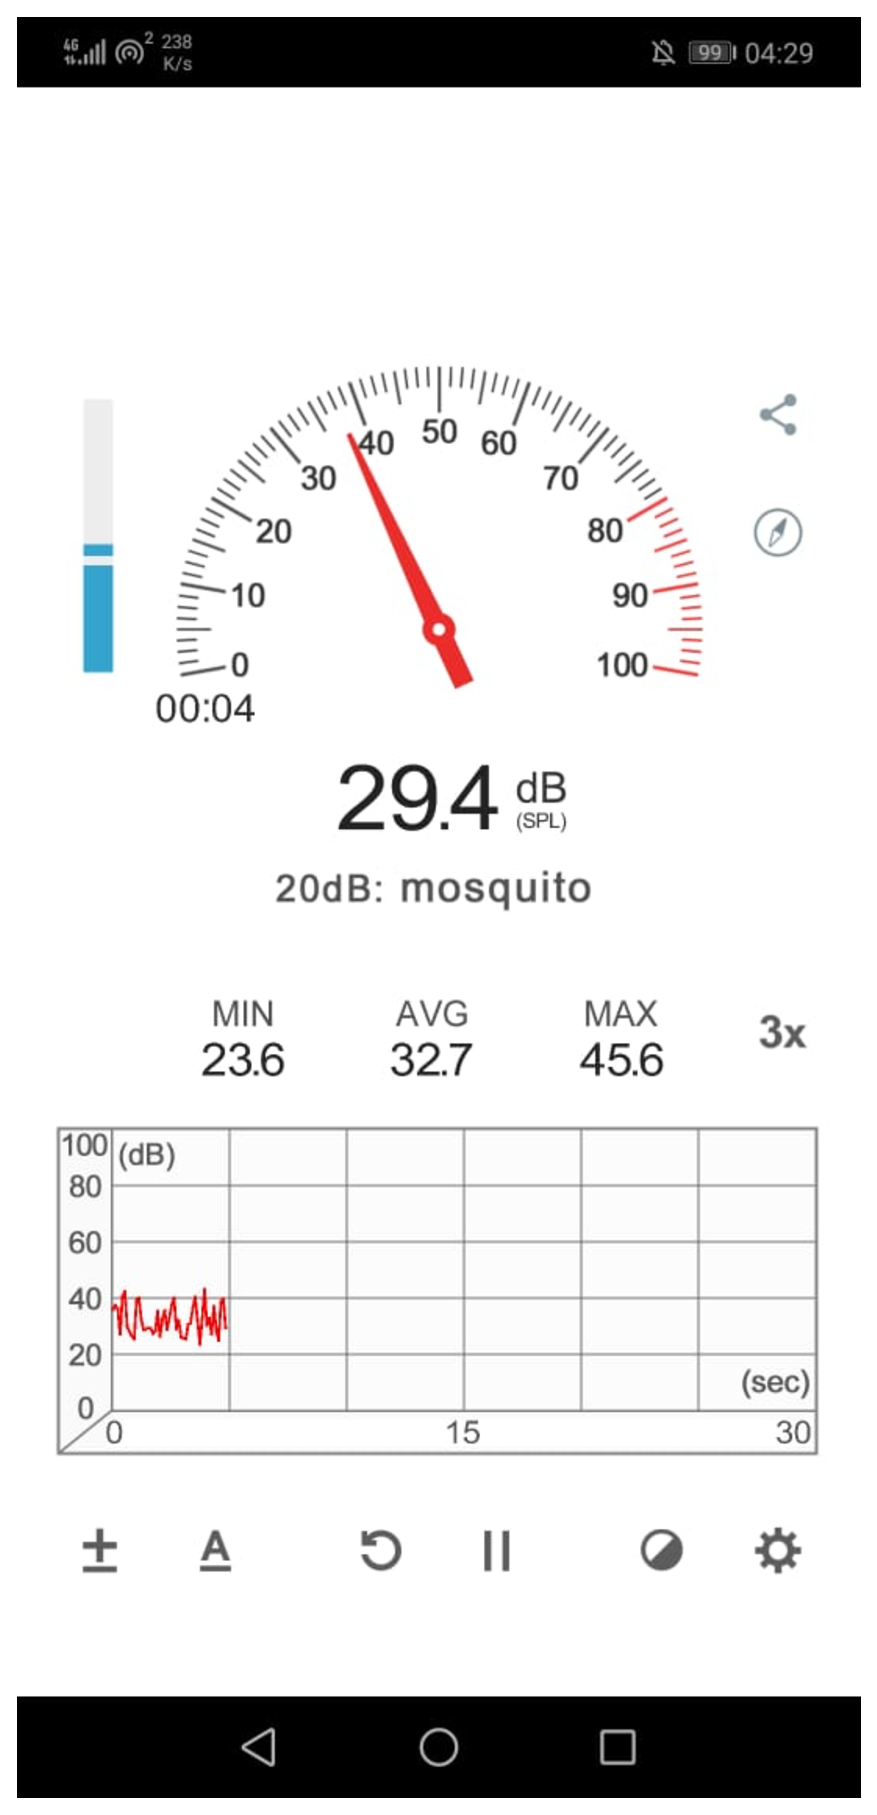
\includegraphics[width=0.28\textwidth]{resources/f4.eps}
\caption{Sonómetro utilizado para la medición.}
\label{figura4}
\source{Elaboración propia.}
\end{figure}

Para facilitar la medición se ha utilizado un sonómetro instalado en un móvil
\emph{Android}, llamada: \textbf{Sonómetro (Sound Meter)}, como puede verse en
la \textbf{Figura \ref{figura4}}.
\\

Una vez localizado en el lugar de medición, se procederá a grabar la pantalla
del móvil durante 7 minutos, y se arrancara la medición con la aplicación. Una
vez terminada la medición se analizará el vídeo para conocer el nivel sonoro
cada $5$ segundos durante $5$ minutos.
\\

Una vez medidos los datos, se procederá a graficar el nivel sonoro vs. tiempo, y
con la ayuda de una \emph{software matemático} se determinara el área que se
encuentra bajo la curva interpolada.
\\

Para determinar el nivel sonoro equivalente $L_{eq}$ se utilizará la siguiente
ecuación:

\begin{equation*}
    L_{eq} = \frac{A_{total}}{t}
\end{equation*}
\vspace{0.10cm}

Finalizando con el análisis del valor equivalente obtenido, según las normativas
vigentes en el país, y municipio.
\\

\textbf{Condiciones de la medición:} \\
\vspace{-0.4cm}

\begin{center}
\begin{tabular}{r|l}
\textbf{Lugar de registro}      & Avenida Blanco Galindo. Km. 4 \textonehalf \tabularnewline
\textbf{Fecha de registro}      & 2021-05-25                                 \tabularnewline
\textbf{Hora de registro}       & Desde 16:32:00 hasta 16:37:00              \tabularnewline
\textbf{Nivel sonoro permitido} & 68 [dB(A)]                                 \tabularnewline
\end{tabular}
\end{center}
\vspace{0.1cm}

\textbf{Croquis de ubicación:} \\

La ubicación geográfica de la medición realizada puede apreciarse en la
\textbf{Figura \ref{figura5}}.

\begin{figure}
\centering
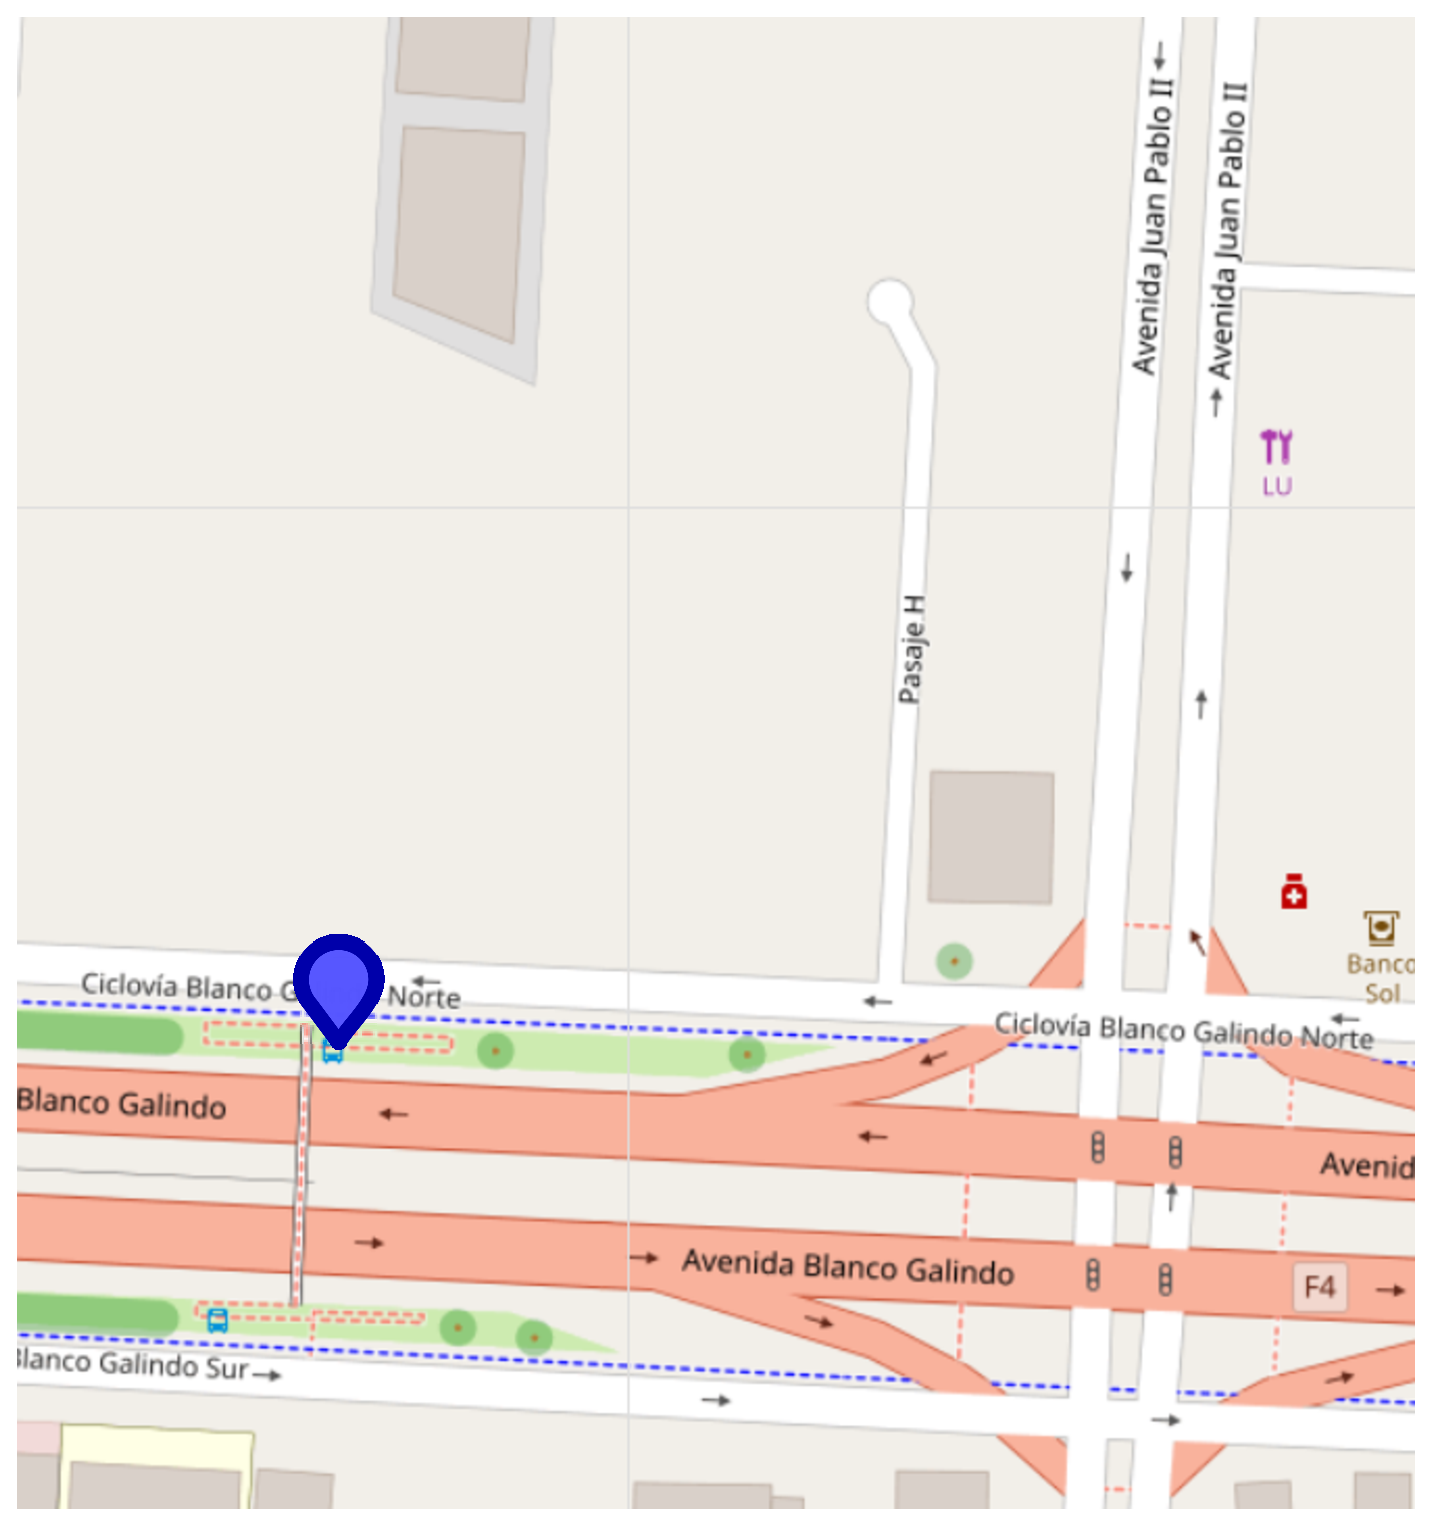
\includegraphics[width=0.75\textwidth]{resources/f5.eps}
\caption{Ubicación geográfica de la medición.}
\label{figura5}
\source{Elaboración propia (a partir del software \emph{OpenStreetMap}).}
\end{figure}
\vspace{0.6cm}

\textbf{Datos tomados en la medición:} \\

En el \textbf{Cuadro \ref{cuadro1}}, se pueden ver los valores medidos del
nivel sonoro.

\begin{table}[!h]
\begin{center}
\begin{tabular}{|c||>{\centering}m{1.2cm}<{\centering}
                   |>{\centering}m{1.2cm}<{\centering}|
                |c||>{\centering}m{1.2cm}<{\centering}
                   |>{\centering}m{1.2cm}<{\centering}|
                |c||>{\centering}m{1.2cm}<{\centering}
                   |>{\centering}m{1.2cm}<{\centering}|}
\hline
$i$ & $t_i [s]$ & $L_i [dB]$ & $i$ & $t_i [s]$ & $L_i [dB]$ &
    $i$ & $t_i [s]$ & $L_i [dB]$
    \tabularnewline \hline \hline
 1 &  0 & 67.4 & 21 & 100 & 69.9 & 41 & 200 & 69.6 \tabularnewline \hline
 2 &  5 & 67.4 & 22 & 105 & 66.6 & 42 & 205 & 68.8 \tabularnewline \hline
 3 & 10 & 65.1 & 23 & 110 & 65.8 & 43 & 210 & 70.6 \tabularnewline \hline
 4 & 15 & 67.2 & 24 & 115 & 71.5 & 44 & 215 & 60.6 \tabularnewline \hline
 5 & 20 & 69.3 & 25 & 120 & 65.4 & 45 & 220 & 67.2 \tabularnewline \hline
 6 & 25 & 65.8 & 26 & 125 & 61.1 & 46 & 225 & 72.3 \tabularnewline \hline
 7 & 30 & 69.5 & 27 & 130 & 66.2 & 47 & 230 & 72.0 \tabularnewline \hline
 8 & 35 & 70.3 & 28 & 135 & 66.0 & 48 & 235 & 68.0 \tabularnewline \hline
 9 & 40 & 72.5 & 29 & 140 & 71.7 & 49 & 240 & 69.3 \tabularnewline \hline
10 & 45 & 84.0 & 30 & 145 & 70.6 & 50 & 245 & 69.5 \tabularnewline \hline
11 & 50 & 77.2 & 31 & 150 & 66.6 & 51 & 250 & 79.6 \tabularnewline \hline
12 & 55 & 77.6 & 32 & 155 & 70.2 & 52 & 255 & 66.8 \tabularnewline \hline
13 & 60 & 74.6 & 33 & 160 & 69.8 & 53 & 260 & 73.0 \tabularnewline \hline
14 & 65 & 78.8 & 34 & 165 & 74.2 & 54 & 265 & 68.9 \tabularnewline \hline
15 & 70 & 76.4 & 35 & 170 & 81.7 & 55 & 270 & 74.2 \tabularnewline \hline
16 & 75 & 71.5 & 36 & 175 & 79.3 & 56 & 275 & 84.4 \tabularnewline \hline
17 & 80 & 71.3 & 37 & 180 & 74.0 & 57 & 280 & 74.0 \tabularnewline \hline
18 & 85 & 71.4 & 38 & 185 & 69.7 & 58 & 285 & 82.5 \tabularnewline \hline
19 & 90 & 84.5 & 39 & 190 & 69.4 & 59 & 290 & 75.7 \tabularnewline \hline
20 & 95 & 81.6 & 40 & 195 & 72.5 & 60 & 295 & 72.2 \tabularnewline \hline
\end{tabular}
\caption{Mediciones de nivel sonoro durante 5 minutos cada 5 segundos.}
\label{cuadro1}
\source{Elaboración propia.}
\end{center}
\end{table}

\section{Resultados}

\begin{figure}
\centering
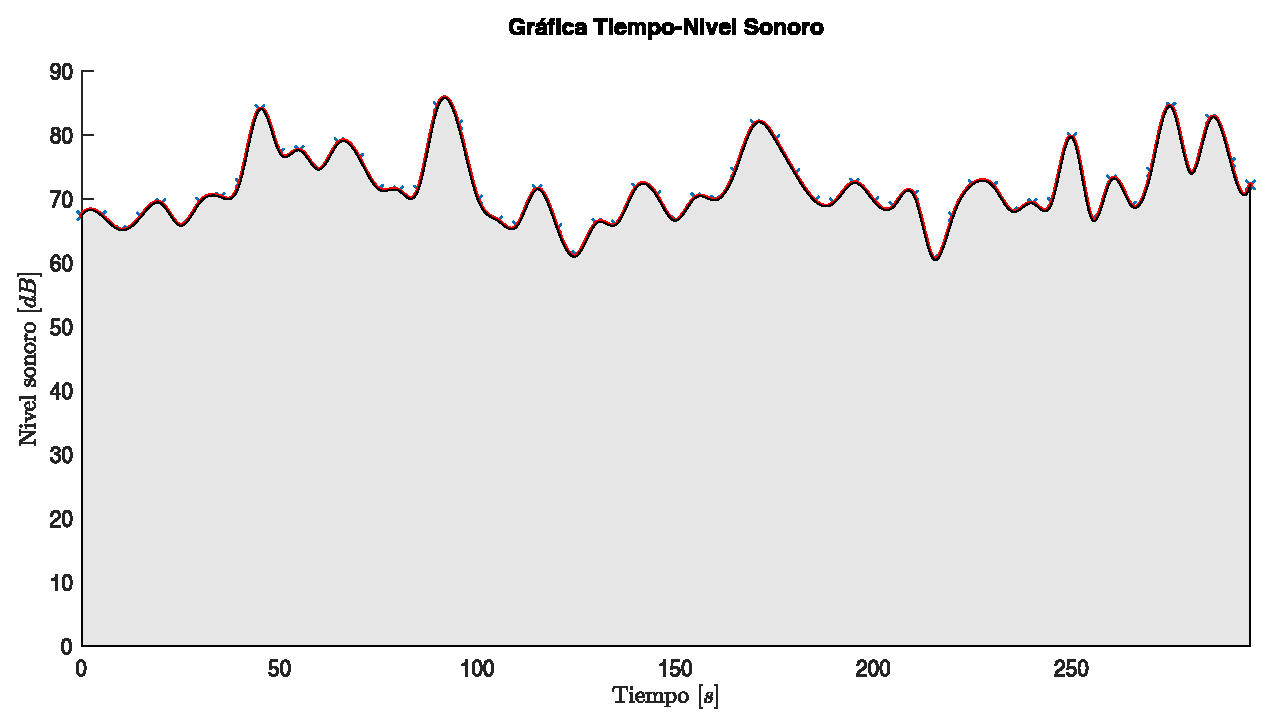
\includegraphics[width=1.0\textwidth]{resources/m1.eps}
\caption{Gráfica de tiempo vs nivel sonoro.}
\label{figura6}
\source{Elaboración propia.}
\end{figure}

A partir de los datos obtenidos y con la ayuda de \emph{Matlab} (véase
\textbf{Apéndice C}) se genera la gráfica de la \textbf{Figura \ref{figura6}},
además de realizar una interpolación polinómica y calcular el área bajo la
curva de tal función en el intervalo $[0,295]$. Resultando ser:

\begin{equation*}
    A_{total} = \num{2.1172e4} [dB\,s]
\end{equation*}
\begin{equation*}
    t = 300 [s]
\end{equation*}
\begin{equation*}
    L_{eq} = \frac{A_{total}}{t} = 70.5735 [dB]
\end{equation*}
\vspace{0.10cm}

El valor hallado supera ligeramente el máximo para fuentes fijas, pero no así
para fuentes móviles; además considerando la tolerancia de $10\%$ permitida por
el reglamento, el ruido en el sitio escogido se encuentra en los margenes
aceptables.

\section{Discusión}

La fiabilidad de una medida de ruido realizada con un móvil puede ser muy baja.
Su precisión depende fundamentalmente de tres factores:

\begin{itemize}
\item La calidad del micrófono (que suele ser mejor en teléfonos de gama alta).
\item La calibración del micrófono (existen algunas \emph{apps} que permiten
    realizarla).
\item La exactitud del software (la aplicación empleada).
\end{itemize}

Estos tres factores por si solos pueden desvirtuar significativamente una
medición de ruido realizada con el móvil. A ellos hay que sumar otros dos que
sólo pueden realizarse con cálculos y programas específicos: la corrección del
ruido de fondo (mayor en entornos ruidosos) y las penalizaciones por los valores
elevados de diferentes componentes del ruido (muy habituales en mediciones de
todo tipo de máquinas) y que pueden suponer un incremento de $9 [dB]$ sobre los
valores medidos.

En conclusión se debe tomar con mucha precaución los valores de medida obtenidos
con un móvil, más cuando estos estén cercanos a los valores límites permitidos
\cite{ALLPE}.

\section{Conclusiones}

Se halló el valor representativo de la medición, resultando este un valor mayor
por menos de $2 [dB]$ al máximo permitido para fuentes de ruido fijo. Pero
siendo menor a todos los valores de fuentes móviles del reglamento.

\begin{thebibliography}{99}

\bibitem{COCHLEA} Sonido: Generalidades.\\
Extraído el 25 de Mayo del 2021, de:\\
{\small \url{https://www.cochlea.eu/es/sonido}.}

\bibitem{PEREZ} Pérez Vega, Constantino.\\
El sonido y la audición.\\
Universidad de Cantabria.\\
Extraído el 25 de Mayo del 2021, de: \\
{\small \url{https://personales.unican.es/perezvr/pdf/sonido%20y%20audicion.pdf}.}

\bibitem{MIGUELMORATEORGANOLOGIA} Nociones básicas sobre acústica musical.\\
Extraído el 25 de Mayo del 2021, de: \\
{\small \url{https://miguelmorateorganologia.wordpress.com/nociones-basicas-de-acustica-musical/}.}

\bibitem{Young&Freedman} Young, Hugh D. y Freedman, Roger A. (2013).\\
Física Universitaria. Volumen 1.\\
13va Edición.\\
Capitulo 16. Sonido y oído

\bibitem{SUPERINTENDENCIA} Superintendencia de riesgos del trabajo.\\
El ruido en el ambiente laboral.\\
Extraído el 25 de Mayo del 2021, de: \\
{\small \url{https://www.srt.gob.ar/wp-content/uploads/2016/08/Guia_practica_2_Ruido_2016.pdf}.}

\bibitem{WIKI1} Decibelio.\\
Extraído el 25 de Mayo del 2021, de: \\
{\small \url{https://es.wikipedia.org/wiki/Decibelio}.}

\bibitem{WIKI2} Ruido acústico.\\
Extraído el 25 de Mayo del 2021, de: \\
{\small \url{https://es.wikipedia.org/wiki/Ruido_ac%C3%BAstico}.}

\bibitem{WIKI3} Contaminación acústica.\\
Extraído el 25 de Mayo del 2021, de: \\
{\small \url{https://es.wikipedia.org/wiki/Contaminaci%C3%B3n_ac%C3%BAstica}.}

\bibitem{ELSEVIER} Peligros del ruido y sus efectos en nuestra salud.\\
Extraído el 25 de Mayo del 2021, de: \\
{\small \url{https://www.elsevier.com/es-es/connect/actualidad-sanitaria/efectos-negativos-del-ruido-y-su-repercusion-en-nuestra-salud}.}

\bibitem{LEY1333} Ley del medio ambiente.\\
Publicada en la Gaceta Oficial de Bolivia el 15 de Junio 1992. \\
Extraído el 25 de Mayo del 2021, de: \\
{\small \url{http://www.oas.org/dsd/fida/laws/legislation/bolivia/bolivia_1333.pdf}.}

\bibitem{ANEXO6} Limites permisibles de emisión de ruido.\\
Extraído el 25 de Mayo del 2021, de: \\
{\small \url{http://museonoelkempff.org/sitio/ACC/Informacion/info/Normas/LimitesPermisiblesEmisionRuido.pdf}.}

\bibitem{ALLPE} Mediciones acústicas.\\
Extraído el 25 de Mayo del 2021, de: \\
{\small \url{https://www.allpe.com/acustica/ingenieria-acustica/mediciones-acusticas/}}

\end{thebibliography}

\newpage
\section*{Apéndice A: Ley No. 1333}
A continuación se detallan todas las consideraciones referentes al ruido en la
Ley No. 1333. Ley del medio ambiente promulgada el 27 de Abril de 1992 y
publicada en la Gaceta Oficial de Bolivia el 15 de Junio 1992.

\begin{enumerate}
\item
\textbf{Ley de medio ambiente.} \\
\textbf{Titulo IV:} De los recursos naturales en general. \\
\textbf{Capitulo III:} Del aire y la atmósfera. \\
\textbf{Articulo 42º.-} El Estado, a través de sus organismos competentes,
establecerá, regulará y controlará los niveles de ruidos originados en
actividades comerciales, industriales, domésticas, de transporte u otras a fin
de preservar y mantener la salud y el bienestar de la población.

\item
\textbf{Reglamento general de gestión ambiental.} \\
\textbf{Titulo III:} De la información ambiental. \\
\textbf{Capitulo VI:} Del sistema nacional de información ambiental. \\
\textbf{Articulo 30º.-} Los elementos principales del medio ambiente que deben
ser recogidos por los centros de información ambiental serán los que estén
relacionados, entre otros, con el estado de las aguas superficiales y
subterráneas, el aire, el suelo, la fauna, la flora, el paisaje, el ruido, los
ecosistemas en general.

Para, ello la red nacional y los centros de información ambiental deberán:

\begin{enumerate}[label=(\alph*)]
\item Promover la realización de estudios y sistematizar la información que
reciban;
\item Analizar periódicamente la evolución de la contaminación y degradación del
medio ambiente;
\item Procesar la información obtenida a fin de proporcionarla a las personas
naturales o colectivas, públicas o privadas, que la soliciten.
\end{enumerate}

\item
\textbf{Reglamento de prevención y control ambiental.} \\
\textbf{Titulo III:} De la evaluación de impacto ambiental. \\
\textbf{Capitulo III:} De la ficha ambiental. \\
\textbf{Articulo 22º.-} El contenido de la FA refleja aspectos relacionados al
proyecto, obra o actividad, tales como:

\begin{itemize}
\item Generación de residuos, de ruido, almacenamiento y manejo de insumos,
posibles accidentes y contingencias.
\end{itemize}

\item
\textbf{Reglamento de prevención y control ambiental.} \\
\textbf{Titulo IV:} Del procedimiento de evaluación de impacto ambiental. \\
\textbf{Capitulo V:} De la declaratoria de impacto ambiental. \\
\textbf{Articulo 85º.-} La Autoridad Ambiental Competente decidirá no conceder
la DIA, con la justificación legal y técnica respectiva, si el proyecto obra o
actividad:

\begin{itemize}
\item Significa la generación o el incremento sinérgico de concentraciones de
contaminantes del aire, el incremento a niveles inadmisibles del ruido y olores,
o la degradación significativa de la calidad del agua.
\end{itemize}

\end{enumerate}

\newpage
\section*{Apéndice B: Anexo 6: Limites permisibles de emisión de ruido
\footnote{Los valores de este Anexo permiten una variación de hasta $+10\%$}}

La unidad práctica de medición del nivel de ruido es el decibelio, conocido como
$dB$. \\

Esta unidad es igual a $20$ veces el logaritmo decimal del cociente de la
presión de sonido ejercida por un sonido medido, y la presión de sonido de un
sonido \emph{estándar} (equivalente a $20$ micropascales). \\

El decibelio (A), conocido como $dB(A)$, es el decibelio medido en una banda de
sonido audible, aplicable a seres humanos. \\

\begin{enumerate}
\item \textbf{Limites permisibles de emisión de ruido proveniente de fuentes
    fijas.} \\

El límite máximo permisible de emisión de ruido en fuentes fijas es de
$68 [dB(A)]$ de las seis a las veintidós horas, y de $65 [dB(A)]$ de las
veintidós a las seis horas. \\

Estos valores deben ser medidos en forma continua o semicontinua en las
colindancias del predio, durante un lapso no menor de quince minutos. \\

Asimismo se debe consideran un límite máximo permisible de emisión de ruido de
$115 [dB(A)]$ mas o menos $3 [dB(A)]$ durante un lapso no mayor a quince minutos
y un valor de $140 [dB(A)]$ durante un lapso no mayor de un segundo. \\

Las fuentes fijas que se localicen en las áreas cercanas a centros
hospitalarios, guarderías, escuelas, asilos y otros lugares de descanso, no
deben rebasar el límite máximo permisible de emisión de ruido de $55 [dB(A)]$.
\\

La instalación de aparatos amplificadores de sonido y otros dispositivos
similares en la vía pública, será autorizada únicamente por la autoridad
competente, cuando el ruido no exceda un nivel de $75 [dB(A)]$. \\

Para la construcción de aeropuertos, aeródromos y helipuertos públicos y
privados, las autoridades competentes deben tener en cuenta la opinión de la
Secretaría Nacional de Salud.

\item \textbf{Limites permisibles de emisión de ruido provenientes de fuentes
    móviles.} \\

El límite máximo permisible de emisión de ruido en fuentes móviles se aplicará
de acuerdo a la siguiente tabla.

\begin{center}
\begin{tabular}{
    |>{\centering}m{4.0cm}<{\centering}|
    |>{\centering}m{2.0cm}<{\centering}
    |>{\centering}m{3.0cm}<{\centering}
    |>{\centering}m{2.0cm}<{\centering}|}
\hline
\textbf{Peso bruto de vehículo} & \textbf{Hasta 3000 [kg]} &
    \textbf{De 3000 [kg] a 100000 [kg]} & \textbf{Mayor a 10000 [kg]} \tabularnewline \hline
\hline
Limite máximo permisible en $[dB(A)]$ & 79 & 81 & 84 \tabularnewline \hline
\end{tabular}
\end{center}
\vspace{0.1cm}

Estos valores deben ser medidos a $15 [m]$ de distancia de la fuente. \\

Para motocicletas, triciclos y cuatriciclos motorizados, el límite máximo
permisible de la emisión de ruido es de $84 [dB(A)]$ y debe ser medido a
$7.5 [m]$ de distancia de la fuente.
\end{enumerate}

\newpage
\section*{Apéndice C: Cálculos realizados en \emph{Matlab}}

A continuación se presenta el código implementado en el programa \emph{Matlab}
para la generación de la gráfica, la interpolación polinómica de los datos, y
el calculo del área bajo la curva.

\begin{shaded}
\begin{alltt}
\footnotesize
\# Datos importados (i1.csv):
\input{resources/i1.csv}

\# Comandos ejecutados (m1.m):
\input{resources/m1.m}
\normalsize
\end{alltt}
\end{shaded}

\newpage
\section*{Apéndice D: Toma de datos}

\begin{figure}
\centering
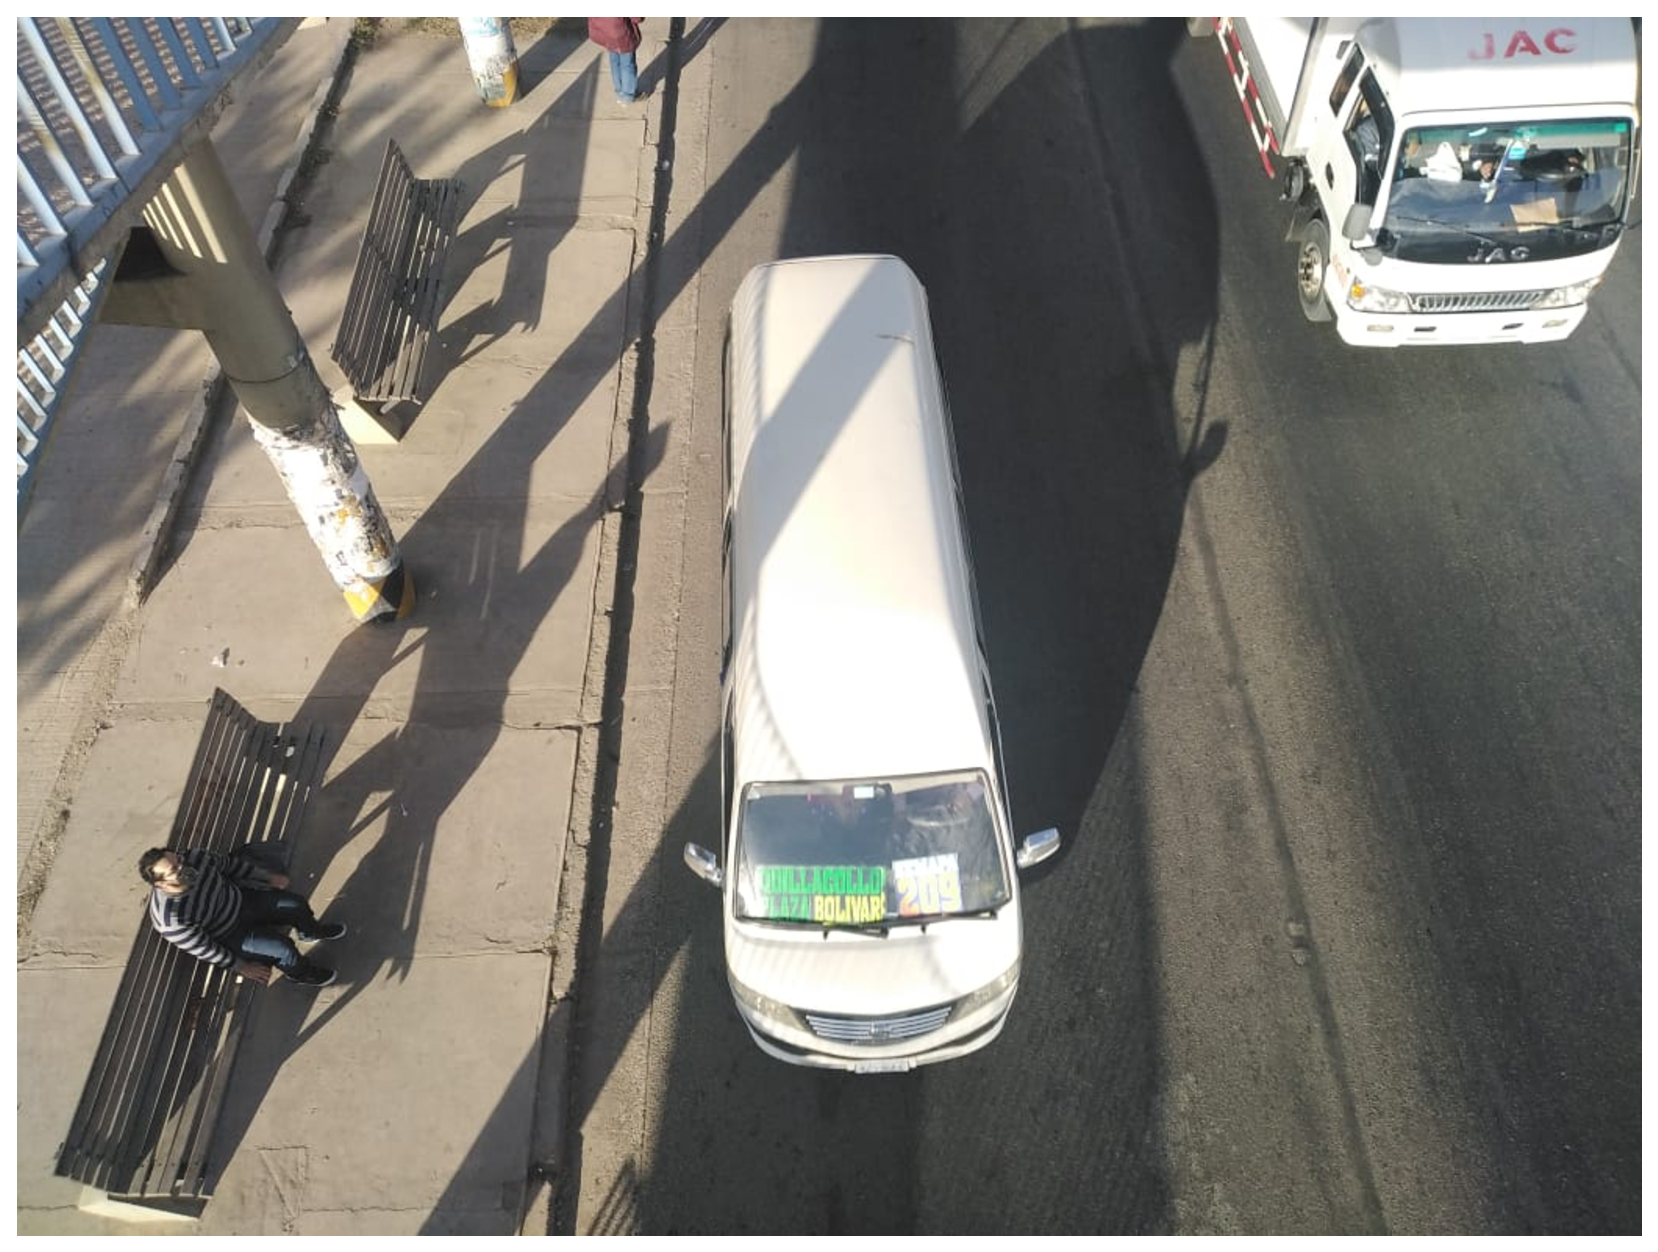
\includegraphics[width=0.90\textwidth]{resources/f7.eps}
\caption{Toma de datos en el punto geográfico escogido.}
\label{figura7}
\source{Elaboración propia.}
\end{figure}

Como comprobación de la autenticidad del trabajo, se adjunta una fotografía del
autor durante la toma de datos, que puede apreciarse en la
\textbf{Figura \ref{figura7}}.

\end{document}

